\documentclass[a4paper]{article}

\usepackage[english]{babel}
\usepackage[utf8]{inputenc}
\usepackage{amsmath}
\usepackage{graphicx}
\usepackage{caption}
%\usepackage{subcaption}
%\usepackage{float}
\usepackage{natbib}
\usepackage{floatrow}
\usepackage[label font=bf,labelformat=simple]{subfig}
\floatsetup[figure]{style=plain,subcapbesideposition=top}
\usepackage[margin=1.25in]{geometry}
\captionsetup{labelfont=bf}
\usepackage{multirow}
\usepackage[table,xcdraw]{xcolor}




\begin{document}

\begin{figure}
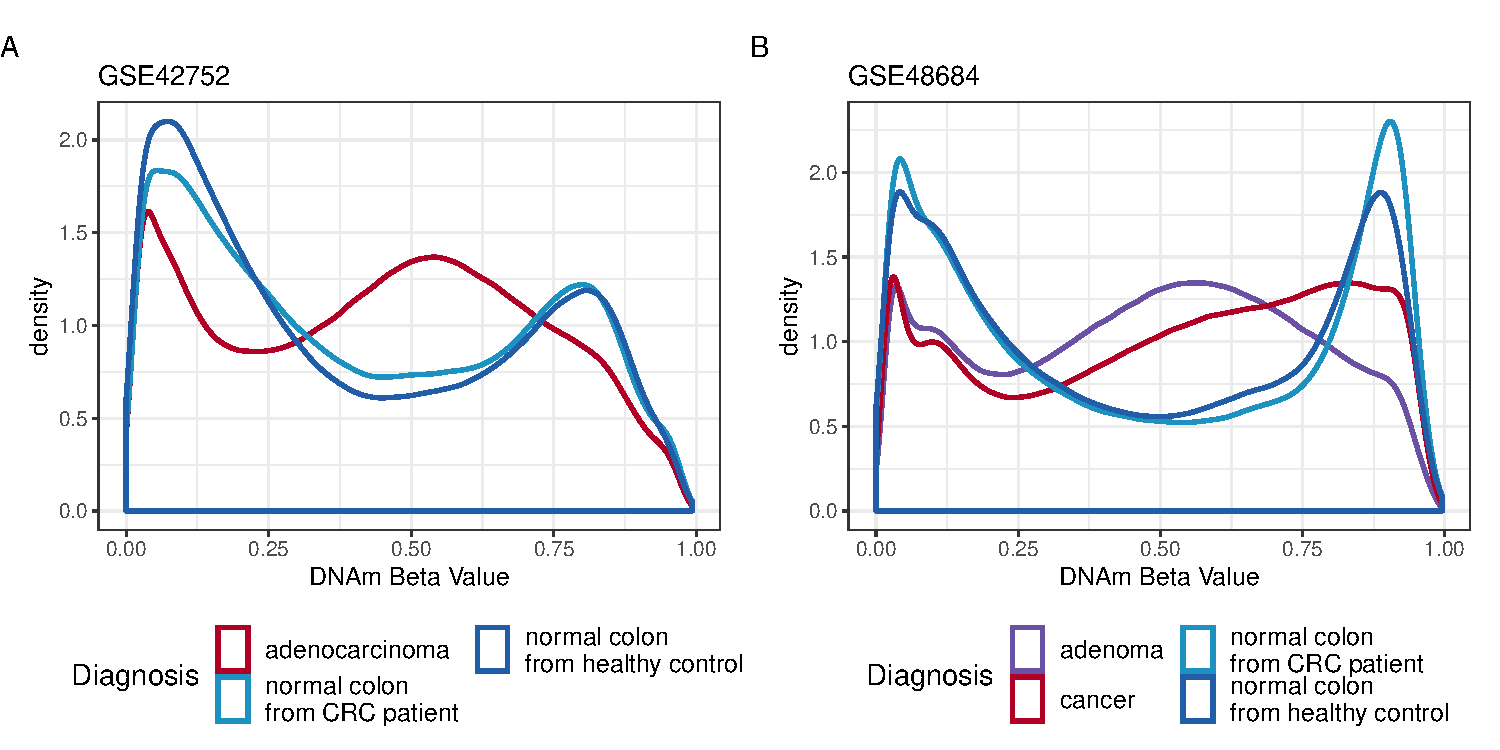
\includegraphics[width=1\textwidth]{../../figs/cancer_public_same_variable_cpg_num.pdf}
\caption{\textbf{Appearance of the trimodal effect in three published cancer datasets.} In all datasets samples grouped by cancer diagnosis, curves show the DNAm distribution the top most variable CpGs. (a) GSE42752; 63 samples; colon samples (b) GSE48684; 147 samples; colon samples (c) GSE53051; 220 samples; For clarity plots are also split into tissue of origin. }
\end{figure}


\begin{figure}
\begin{centering}
\sidesubfloat[]{\label{main:A}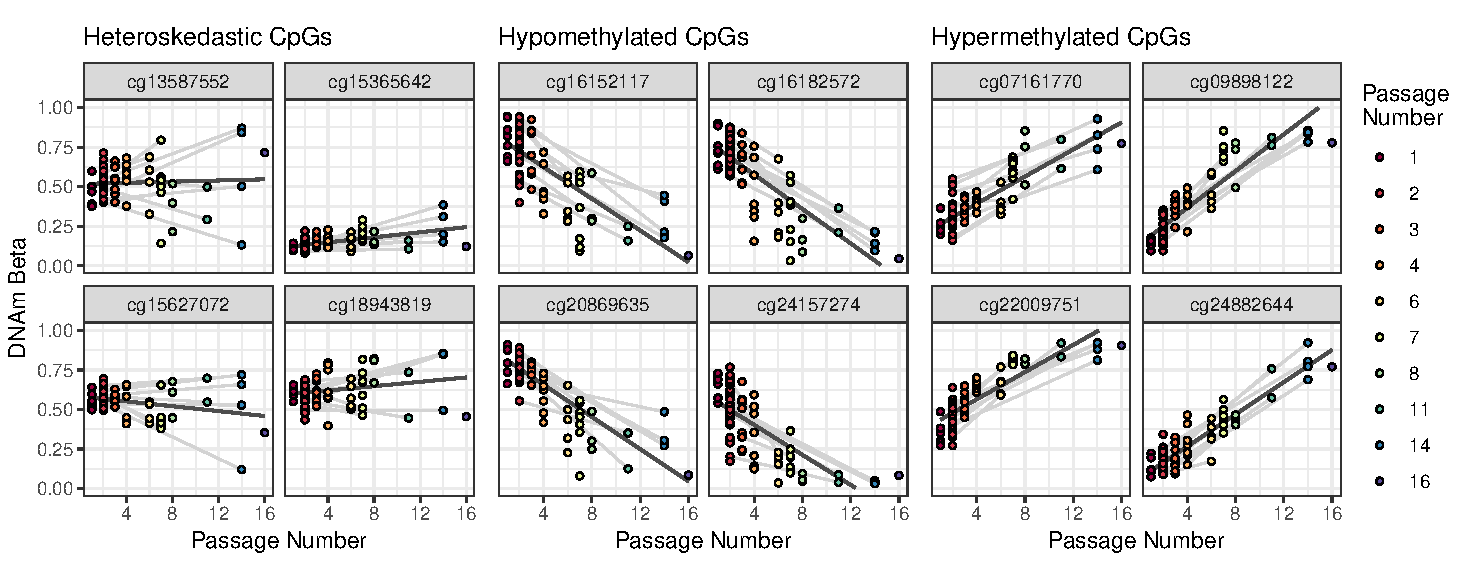
\includegraphics[width=1\textwidth]{../../figs/Passage_representative_CpGs_FDR.pdf}}
\hfil
\sidesubfloat[]{\label{main:B}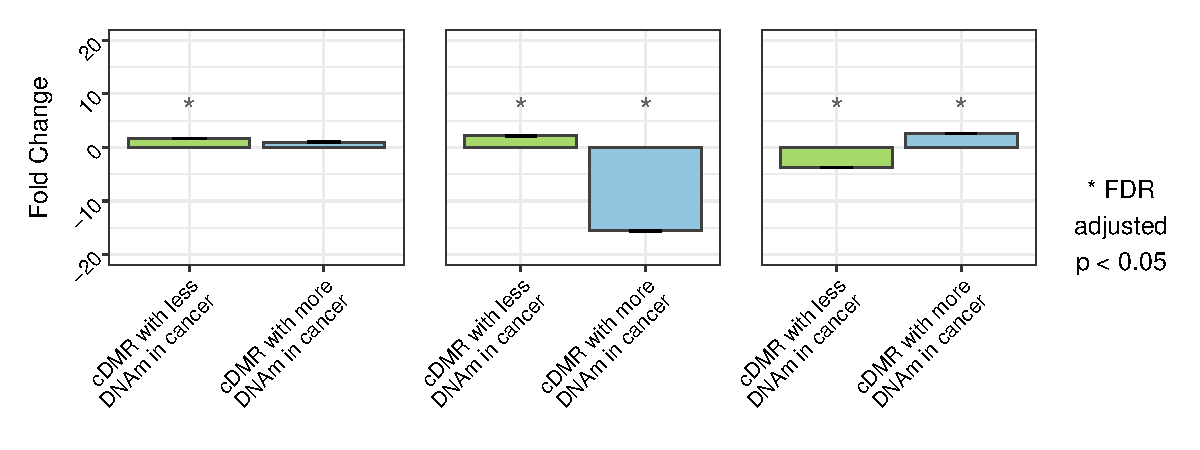
\includegraphics[width=1\textwidth]{../../figs/Passage_hetero_hypo_hyper_DMR_CpGs_FDR_background015.pdf}}

\caption{\textbf{Passage affects DNAm in specific regions of the genome.} (a) Representative CpGs with DNAm significantly associated to passage. CpGs were selected that are either significantly heteroskedastic with passage or are differentially DNA methylated and either lose (hypomethylated) or gain (hypermethylated) DNAm with increasing passage. Samples are coloured by passage number and grey lines connect samples derived from the same patient. Regression lines between passage and DNAm are in black.(c) Fold change between the number of passage associated CpGs in cDMRs and expected number based on the EPIC array background. Standard error bars around the mean fold change are for the error between 1,000 random samplings.}

\label{fig:main}
\end{centering}
\end{figure}







\end{document}